\documentclass{../class/tecnia-uni-article}

\usepackage[utf8]{inputenc}

\usepackage{lipsum}
\usepackage{graphicx}

\addbibresource{myreferences.bib}

\SetTecniaDoiNumber{10.12356/tecnia.vxxxx.xxx}
\SetTecniaVolDate{Vol\textbf{.xx} N°\textbf{y} \textbf{Enero-Junio 202x}}
\SetTecniaInitialPage{3}
\SetTecniaAuthorEtAl{Author et al.}


\begin{document}


\twocolumn[{%
\TecniaTitleFormat{Un título muy grande creado solo para probar el comportamiento de espaciado}
\TecniaTitleFormat{A very large title created only to test the spacing behavior}
%
%
\begin{TecniaAuthors}
\TecniaAuthorFormat{Fernando Pujaico Rivera}{1}{https://orcid.org/0000-0002-4970-2818}
\textbf{,}  
\TecniaAuthorFormat{John Doe}{2}{}
\textbf{,} 
\TecniaAuthorFormat{Jane Doe}{2}{}
\end{TecniaAuthors}
%
%
\begin{TecniaInstitutions}
\TecniaInstitution{1}{Universidad nacional de Ingenieria}
\textbf{,} 
\TecniaInstitution{2}{UNICAMP}
\end{TecniaInstitutions}
%
%
\begin{TecniaDate}
Received: November 07, 2022 - Accepted: March 03, 2023
\end{TecniaDate}
%
%
\rule{\textwidth}{1pt}\\[0mm]
%
%
\begin{TecniaAbstract}{Resumen}
\lipsum[1]
\end{TecniaAbstract}
%
%
\begin{TecniaKeywords}{Palabras Clave}
palavra1, palavra2, palavra3, palavra4.
\end{TecniaKeywords}\\[0mm]
%
%
\begin{TecniaAbstract}{Abstract}
\lipsum[1]
\end{TecniaAbstract}
%
%
\begin{TecniaKeywords}{Keywords}
palavra1, palavra2, palavra3, palavra4.
\end{TecniaKeywords}
%
%
\rule{\textwidth}{1pt}\\[0mm]
}]


%%%%%%%%%%%%%%%%%%%%%%%%%%%%%%%%%%%%%%%%%%%%%%%%%%%%%%%%%%%%%%%%%%%%%%%%%%%%%%%%%%%%%%%%%%%%%%%%%
\section{A very large title section name}

\lipsum[1-2]
\begin{figure}[!ht]
  \centering
  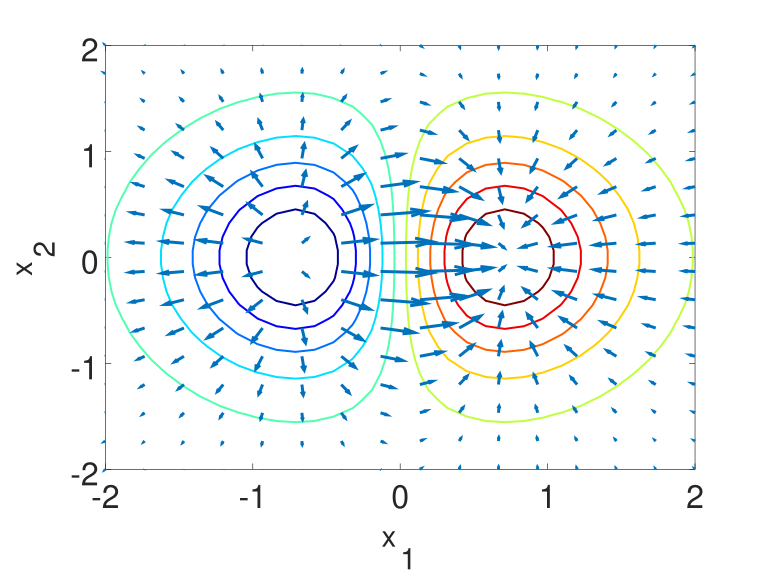
\includegraphics[width=0.85\linewidth]{screenshot.png}
  \caption{A picture of Lena}
\end{figure}
\lipsum[1]. See the Eq. \ref{eq:1} or \ref{eq:2}
\begin{equation}\label{eq:1}
x=\sum_{n}^{N}a^{n}
\end{equation}
\lipsum[1] $x+y+z=0$ some text $x=\sum_{n}^{N}a^{n}$ \lipsum[1] 
\begin{equation}\label{eq:2}
y=\sum_{n}^{N}b^{n}
\end{equation}

%%%%%%%%%%%%%%%%%%%%%%%%%%%%%%%%%%%%%%%%%%%%%%%%%%%%%%%%%%%%%%%%%%%%%%%%%%%%%%%%%%%%%%%%%%%%%%%%%
\section{Title of section}
\lipsum[1] 
Table \ref{table:1} is an example of a referenced \LaTeX{} element.

\begin{table}[h!]
\centering
\caption{Table to test captions and labels.}
\label{table:1}
\begin{tabular}{cccc} 
 \hline
 Col1 & Col2 & Col2 & Col3 \\ [0.5ex] 
 \hline\hline
 1 & 6 & 87837 & 787 \\ 
 2 & 7 & 78 & 5415 \\
 3 & 545 & 778 & 7507 \\
 4 & 545 & 18744 & 7560 \\
 5 & 88 & 788 & 6344 \\ [1ex] 
 \hline
\end{tabular}
\end{table}
\lipsum[1]

%%%%%%%%%%%%%%%%%%%%%%%%%%%%%%%%%%%%%%%%%%%%%%%%%%%%%%%%%%%%%%%%%%%%%%%%%%%%%%%%%%%%%%%%%%%%%%%%%
\section{Conclusion}
\lipsum[1] \cite{texbook} \cite{latex:companion}


%%%%%%%%%%%%%%%%%%%%%%%%%%%%%%%%%%%%%%%%%%%%%%%%%%%%%%%%%%%%%%%%%%%%%%%%%%%%%%%%%%%%%%%%%%%%%%%%%


\printbibliography[title=References]

\end{document}














